%  !TeX  root  =  user_guide.tex

\section{OpenStreetMap Plugin}\label{plugins_osm}

% when the revision of a section has been finalized,
% comment out the following line:
% \updatedisclaimer

In recent years the OpenStreetMap project has gained popularity because in
many countries no free geo data such as digital roadmaps are available.
Target of the OSM project is to create a free editable map of the world
from GPS data, aerial photography or simply from local knowledge. To
support this idea QGIS provides a plugin that enables its users to work
with OSM data.

The plugin provides all basic functionalities for OSM data manipulation,
such as data loading, importing, saving, downloading, editing and
uploading data back to the OpenStreetMap server. While implementing OSM
plugin an inspiration was taken from existing OSM data editors. The
purpose was to combine their functionalities to get the best
possible result.

The following section gives a brief introduction to principles of the OSM
project. If you are not interested in information on OSM just skip the next
section. Parts of the following paragraphs are copied from the
OpenStreetMap web site at \url{http://www.openstreetmap.org}.

\minisec{The OpenStreetMap project}

OpenStreetMap is a project to create a free editable map of the world. The
maps are created using data from portable GPS devices, aerial photography,
other free sources or simply from local knowledge. The project was started
because most maps have legal or technical restrictions on their use, holding
back people from using them in creative, productive, or unexpected ways. Both
rendered images and the vector dataset of OSM are available for download
under a Creative Commons Attribution ShareAlike 2.0 licence.

\begin{figure}[ht]
   \centering
   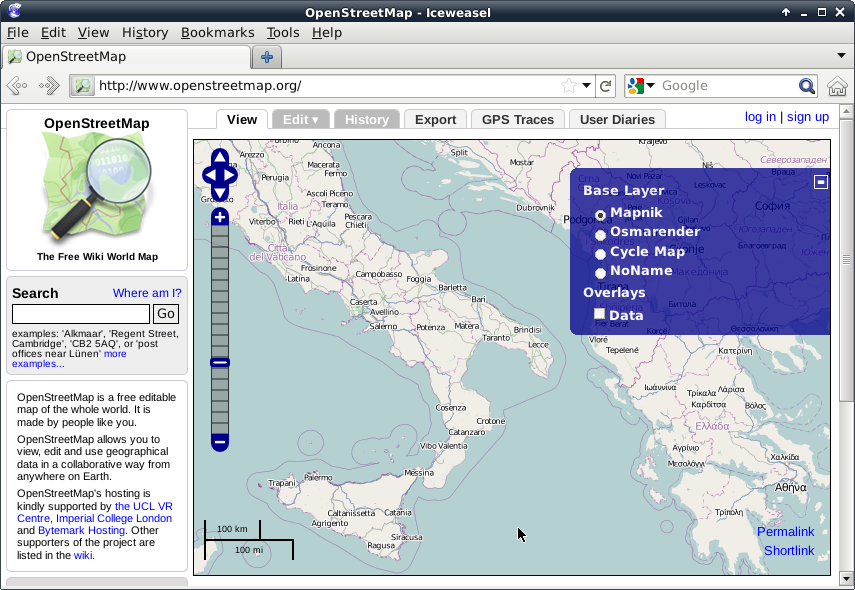
\includegraphics[clip=true, width=10cm]{osmweb}
   \caption{OpenStreetMap data in the web \nixcaption}\label{fig:osmweb}
\end{figure}

OpenStreetMap was inspired by sites such as Wikipedia - the map display
(see Figure \ref{fig:osmweb}) features a prominent \tab{Edit} tab and a
full revision history is maintained. Registered users can upload GPS track
logs and edit the vector data using the given editing tools.

OSM data primitive is an object class that can be stored via the API in the
server. The three supported types of data are: \textbf{Node}, \textbf{Way}
and \textbf{Relation}.

\begin{itemize}[label=--]
\item \textbf{A node} is a latitude/longitude pair of coordinates. It is
used as building a block for other features and as a feature itself (Points
Of Interest), if they are tagged as required.
\item \textbf{A way} is a list of at least two nodes that describe a linear
feature such as a street, or similar. Nodes can be members of multiple ways.
\item \textbf{A relation} is a group of zero or more primitives with
associated roles. It is used to specify relationships between objects,
and may also model an abstract object.
\end{itemize}

Several different logical features in a common map ('Point Of Interest',
'Street', 'Tram Line', 'Bus Stop' etc.) are defined by these primitives.
Map features are well-known in the OSM community and are stored as tags,
based of a key and a value. OSM is usually distributed in XML format. XML
payload is used for the communication with the OSM server as well.

\minisec{QGIS - OSM Connection}\label{qgis-osm-connection}

The first part of this section describes how OSM data primitives
are displayed in QGIS vector layers. As written above, OSM data consist of
Nodes, Ways and Relations. In QGIS they are displayed in three different
layer types: Point layer, Line layer and Polygon layer. It's not possible
to remove any of these layers and work with the other ones.

\begin{itemize}[label=--]
\item A \textbf{Point layer} displays all features of type Node that stands
alone. That means that only Nodes that are not included in any Way belongs
to the Point layer.
\item A \textbf{Line layer} displays those OSM features of type Way that are
not closed. That means, none of these Ways starts and ends with the
same Node.
\item A \textbf{Polygon layer} displays all Ways that are not included in
Line layer.
\end{itemize}

OpenStreetMap has one more data primitive except for the three mentioned
above. This is called \textbf{Relation}. There is purposely no vector layer
to display Relations. A Relation defines relation between any number of
data primitives. After Point, Line or Polygon is identified on a map,
the plugin shows a list of all relations, the identified feature is part of.

Challenging was to design the connection between OSM data and the
standard QGIS editing tools. These tools are made to edit a single vector
layer at a time, no matter of what feature types it displays. This means
that if OSM data are loaded to QGIS through the plugin, you could
(theoretically) edit Point layer, Line layer or Polygon layer with these
standard tools separately.

The problem is, that Line layer consists of two different types of OSM
features - Ways and Nodes. Why? Because in OSM format a Way is composed of
Nodes. If you start editing a Line layer and change the shape of some line,
your action must affect not only the OSM Way but also the OSM Nodes that
are part of it.

QGIS standard editing tools cannot tell the OSM provider, which members
of which line has changed and how. It can tell only what's the new geometry
of which line, and that's not enough to propagate changes to the OSM database
correctly. The Line layer does also not know the identifiers of the line
members. The same problem occurs when you try to edit the Polygon layer.

For this reason, the OSM plugin need its own tools for editing OSM data.
While they are used, the OSM layers can be changed correctly. The Plugin
editing tools consists of tools for Point, Line, Polygon and
Relation creation, deletion and moving.

\textbf{Note:} To create a connection between the OSM plugin and standard
editing tools, changes in QuantumGIS core code would be necessary.

\subsection{Installation}

The OpenStreetMap plugin is a core plugin inside QGIS. If you have python
support enabled, the 'OpenStreetMap' plugin can be selected in the Plugin
Manager as described in section \ref{sec:load_core_plugin}).

\subsection{Basic user interface}

The first time the OSM plugin is started (and after the first data are
loaded), several new OSM plugin icons appear in the QGIS toolbar menu
together with new graphical components as shown in Figure
\ref{fig:osmwidget}:

\begin{figure}[ht]
   \centering
   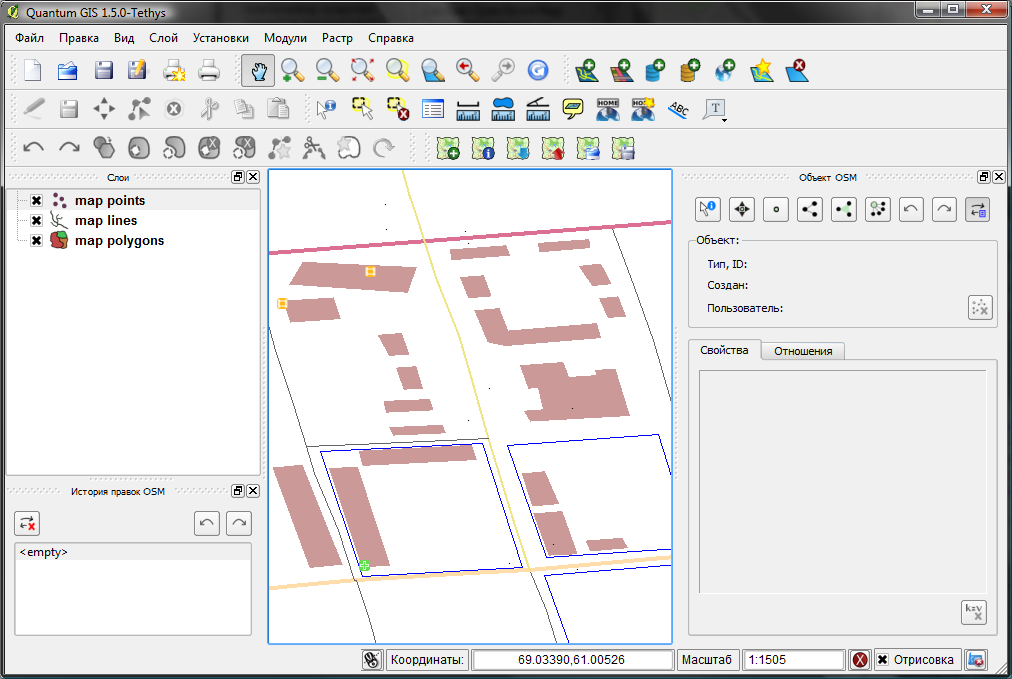
\includegraphics[clip=true, width=10cm]{osm_widgets}
   \caption{OSM plugin user interface \nixcaption}\label{fig:osmwidget}
\end{figure}

\minisec{OSM Features widget}

The OSM Feature widget helps to identify OSM features. It
shows basic information on feature type and identifier as well as info on
who has when changed a feature. The OSM Feature widget also provides all
editing tools (in the top part of it). More information on those tools can be
found in the sections below. The widget is initially disabled. It
activates itself after successful loading some OSM data.

\minisec{OSM Undo/Redo widget}

This Undo/Redo widget is used to undo and redo edit actions. It consists
not only of a classical Undo and Redo button, it also shows a list with a
brief description of the edit actions that were done. The OSM Undo/Redo
widget is initially closed. You can show it using a button on OSM Feature
widget.

\minisec{Toolbar menu icons}

\begin{description}
\item \toolbtntwo{osm_load}{Load OSM from file}: is used to load data from a
special OpenStreetMap XML file.
\item \toolbtntwo{osm_featureManager}{Show/Hide OSM Feature Manager} is
used to show or hide the OSM Feature widget. The OSM Feature widget is a
panel that helps with OSM feature identification and with OSM data editing.
\item \toolbtntwo{osm_download}{Download OSM data} is used to download data
from the OpenStreetMap server.
\item \toolbtntwo{osm_upload}{Upload OSM data} is used to upload changes
(on current data).
\item \toolbtntwo{osm_import}{Import data from a layer} is used to import
data from a vector layer. At least one vector layer must be loaded and
current OSM data must be selected.
\item \toolbtntwo{osm_save}{Save OSM to file} is used to save OSM data
back to an XML file.
\end{description}

More detailed information on all the widgets, buttons and dialogs can be
found in appropriate sections of this plugin section according to their
functionality (editing, identification, etc.).

\subsection{Loading OSM data}

The first action that should be done after starting the OSM Plugin is
opening data from an OSM file. OSM data can be import as shapefile or
downloaded directly from the OpenStreetMap server. Here we are focusing
on the first mentioned method.

To load data from a file use the \toolbtntwo{osm_load}{Load OSM from file}
icon. If there is no such button, maybe someone disabled OpenStreetMap
toolbar in your QGIS installation. You can enable it again selecting
\mainmenuopt{Settings} \arrow \mainmenuopt{Toolbars} \arrow \dropmenuopt{OpenStreetMap}.

\begin{figure}[ht]
   \centering
   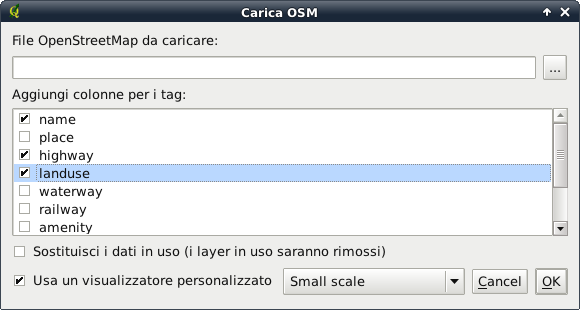
\includegraphics[clip=true, width=10cm]{osmloaddialog}
   \caption{Load OSM data dialog \nixcaption}\label{fig:osmload}
\end{figure}

Purpose of its elements is explained below.

\begin{description}
\item \textbf{OpenStreetMap file to load}: Click on the button to select
the .osm file you want to load data from.
\item \textbf{Add columns for tags}: This option determines a connection
between OSM and QGIS data. Each feature of OSM data has
some tags (pairs of key and value), that define the feature properties.
Each feature of a QGIS vector layer also has its attributes (key and value).
With this option you can define which properties of OSM objects should
be visible when displaying detailed information about QGIS features.
\item \textbf{Replace current data}: Checking this option means that
new data should replace current data the user is working with. Layers of
current data will be removed and new ones will be loaded. When loading
OSM data for the first time, this option is not active, because there is
nothing to replace.
\item \textbf{Use custom renderer}: This option determines how many details
of the map will be used. There are three pre-defined OSM styles for map
displaying. Use \button{Small scale} if you want to view OSM data at low level,
to see all details and to edit something. If not you can use
\button{Medium scale} or \button{Large scale}. QGIS \CURRENT doesn't
support changing the renderer style dynamically.
\end{description}

Click \button{Ok} to load your data. If this is the first time OSM
file is loaded, the plugin must first parse the database. This may take few
seconds or minutes - it depends on the amount of loaded data.

\subsection{Viewing OSM data}

After OSM data are loaded, you can identify map features using the
appropriate tool. Use the \toolbtntwo{osm_identify}{Identify feature}
button on the top-left of OSM Feature widget. Using this tool you can
easily explore all map objects. When the mouse cursor is placed over an
object, you can see all information on it directly in the OSM Feature widget.
There is also a dynamic rubberband displayed on the map so that the user
is able to determine which feature is currently identified.

The \tab{Properties} tab of the widget contains of all feature tags.
Clicking on the \tab{Relation} tab shows you a list of all relations
connected with identified feature.

If you want to hold a feature for a while to be able to read its properties
and relations, move the mouse cursor at the same time, try left-clicking
while you are over the feature. Identification process will stop until next
left-clicking.

Sometimes there are more than one feature at a point where left-clicking
was performed. This happens especially when clicking on cross-roads or if
you didn't zoom enough into the map. In this situation only one of such
features is identified (and marked with the rubberband) but the plugin
remembers all of them. Then (still in the pause mode) you can change
identified features cyclical with right-clicking.

\subsection{Editing basic OSM data}

In the title of this section 'basic data' means non-relation OSM features -
nodes and ways. If you prefer reading information on relation editing, just
skip this section and read the next one.

Basic data editing is a key part of OSM Plugin. You can change property,
position or shape of any existing basic feature. You can remove features or
add new ones. All such changes on nodes and ways are remembered for
comfortable usage of Undo/Redo operations and for easy upload of all changes
to OpenStreetMap server.

\minisec{Changing feature tags}

Changing the property/tag of an OSM feature can be done directly in
the table of feature tags. The Tags table of basic features can be found
on the OSM Feature widget. Don't forget to identify feature first.

\begin{figure}[ht]
   \centering
   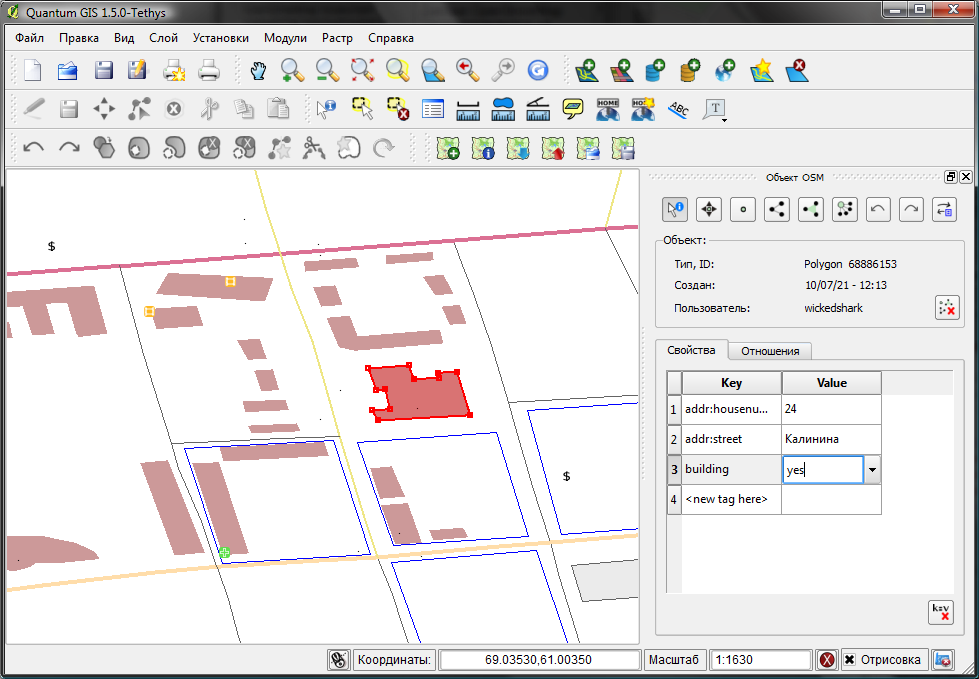
\includegraphics[clip=true, width=12cm]{osm_changefeaturetag}
   \caption{Changing an OSM feature tag \nixcaption}\label{fig:osmchfeattag}
\end{figure}

If you want to change a tag value, just double-click in the appropriate row of
column 'Value' and type or select a new value. If you want to remove a tag,
click in its row, then use button \button{Remove selected tags} on the right
bottom under the table.

To add new tags just type its key and value into the last row of the table -
where '<next tag value>' is written. Notice that you cannot change the key of
an existing tag pair. For comfortable usage, there are some combo boxes of all
existing tag keys and their typical values.

\minisec{Point creation}

For point creation there is a \toolbtntwo{osm_createPoint}{Create point}
button on the OSM Feature widget. To create some points just click on the
button and start clicking on the map. If your cursor is over some map
feature, the feature is marked/identified immediately. If you click on
the map when a line or polygon is marked, a new point is created directly on
such line or polygon - as its new member. If your cursor is over an existing
point, new point cannot be created. In such case the OSM plugin will show
following message:

\begin{figure}[ht]
   \centering
   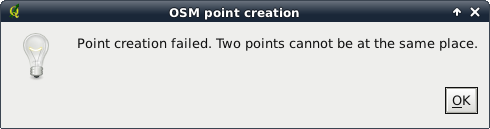
\includegraphics[clip=true, width=8cm]{osm_pointcreation}
   \caption{OSM point creation message \nixcaption}\label{fig:osmpoicreat}
\end{figure}

The mechanism of helping a user to hit the line or polygon is called snapping
and is enabled by default. If you want to create a point very close to some
line (but not on it) you must disable snapping by holding the
\keystroke{Ctrl} key first.

\minisec{Line creation}

For line creation there is a \toolbtntwo{osm_createLine}{Create line} button
on the OSM Feature widget. To create a line just click the button and start
left-clicking on the map. Each of your left-clicks is remembered as a member
vertex of the new line. Line creation ends when first right-click is performed.
The new line will immediately appear on the map.

\textbf{Note}: A Line with less than two members cannot be created. In
such case the operation is ignored.

Snapping is performed to all map vertices - points from Point vector layer
and all Line and Polygon members. Snapping can be disabled by holding the
\keystroke{Ctrl} key.

\minisec{Polygon creation}

For polygon creation there is a \toolbtntwo{osm_createPolygon}{Create polygon}
button on the OSM Feature widget. To create a polygon just click the button
and start left-clicking on the map. Each of your left-clicks is remembered as
a member vertex of the new polygon. The Polygon creation ends when first
right-click is performed. The new polygon will immediately appear on the map.
Polygon with less than three members cannot be created. In such case
operation is ignored. Snapping is performed to all map vertexes - points
(from Point vector layer) and all Line and Polygon members. Snapping can be
disabled by holding the \keystroke{Ctrl} key.

\minisec{Map feature moving}

If you want to move a feature (no matter what type) please use the
\toolbtntwo{osm_move}{Move feature} button from the OSM Feature widget menu.
Then you can browse the map (features are identified dynamically when you
go over them) and click on the feature you want to move. If a wrong feature is
selected after your click, don't move it from the place. Repeat right-clicking
until the correct feature is identified. When selection is done and you move
the cursor, you are no more able to change your decision what to move.
To confirm the move, click on the left mouse button. To cancel a move, click
another mouse button.

If you are moving a feature that is connected to another features, these
connections won't be damaged. Other features will just adapt themselves to
a new position of a moved feature.

Snapping is also supported in this operation, this means:

\begin{itemize}[label=--]
\item When moving a standalone (not part of any line/polygon) point,
snapping to all map segments and vertices is performed.
\item When moving a point that is a member of some lines/polygons,
snapping to all map segments and vertices is performed, except for
vertices of point parents.
\item When moving a line/polygon, snapping to all map vertices is performed.
Note that the OSM Plugin tries to snap only to the 3 closest-to-cursor
vertices of a moved line/polygon, otherwise the operation would by very slow.
Snapping can be disabled by holding \keystroke{Ctrl} key during the operation.
\end{itemize}

\minisec{Map feature removing}

If you want to remove a feature, you must identify it first. To remove
an identified feature, use the \toolbtntwo{osm_removeFeat}{Remove this
feature} button on the OSM Feature widget. When removing a line/polygon,
the line/polygon itself is deleted, so are all its member points that
doesn't belong to any other line/polygon.

When removing a point that is member of some lines/polygons, the point is
deleted and the geometries of parent lines/polygons are changed. The new
parent geometry has less vertices than the old one.

If the parent feature was a polygon with three vertexes, its new geometry
has only two vertexes. And because there cannot exist polygon with only two
vertices, as described above, the feature type is automatically changed to
Line.

If the parent feature was a line with two vertexes, its new geometry has
only one vertex. And because there cannot exist a line with only one vertex,
the feature type is automatically changed to Point.

\subsection{Editing relations}\label{editing_osm_relation}

Thanks to existence of OSM relations we can join OSM features into groups and
give them common properties - in such way we can model any possible map
object: borders of a region (as group of ways and points), routes of a bus,
etc. Each member of a relation has its specific role. There is a pretty good
support for OSM Relations in our plugin. Let's see how to examine, create,
update or remove them.

\minisec{Examining relation}\label{examrelation}

If you want to see relation properties, first identify one of its members.
After that open the \tab{Relations} tab on the OSM Feature widget. At the
top of the tab you can see a list of all relations the identified feature
is part of. Please choose the one you want to examine and look at its
information below. In the first table called 'Relation tags' you find the
properties of the selected relation. In the table called 'Relation members'
you see brief information on the relation members. If you click on a member,
the plugin will make a rubberband on it in the map.

\minisec{Relation creation}

There are 2 ways to create a relation:

\begin{enumerate}
\item You can use the \toolbtntwo{osm_createRelation}{Create relation}
button on OSM Feature widget.
\item You can create it from the \tab{Relation} tab of OSM Feature widget
using the \toolbtntwo{osm_addRelation}{Add relation} button.
\end{enumerate}

In both cases a dialog will appear. For the second case, the feature that
is currently identified is automatically considered to be the first
relation member, so the dialog is prefilled a little. When creating
a relation, please select its type first. You can select one of
predefined relation types or write your own type. After that fill the
relation tags and choose its members.

If you have already selected a relation type, try using the
\toolbtntwo{osm_generateTags}{Generate tags} button. It will generate typical
tags to your relation type. Then you are expected to enter values to the
keys. Choosing relation members can be done either by writing member
identifiers, types and roles or using the \toolbtntwo{osm_identify}{identify}
tool and clicking on map.

Finally when type, tags and members are chosen, the dialog can be submitted.
In such case the plugin creates a new relation for you.

\minisec{Changing relation}

If you want to change an existing relation, identify it first (follow steps
written above in Section 'Examining relation'). After that click on the
\toolbtntwo{osm_editRelation}{Edit relation} button. You will find it
on the OSM Feature widget. A new dialog appears, nearly the same as for the
'create relation' action. The dialog is pre-filled with information on
given relations. You can change relation tags, members or even its type.
After submitting the dialog your changes will be committed.

\subsection{Downloading OSM data}

To download data from OpenStreetMap server click on the
\toolbtntwo{osm_download}{Download OSM data} button. If there is no
such button, the OSM toolbar may be disabled in your QGIS instalation.
You can enable it again at \mainmenuopt{Settings} \arrow
\mainmenuopt{Toolbars} \arrow \dropmenuopt{OpenStreetMap}. After clicking the
button a dialog occurs and provides following functionalities:

\begin{figure}[ht]
   \centering
   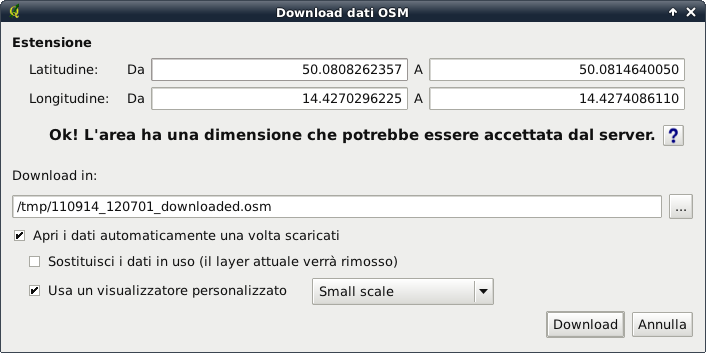
\includegraphics[clip=true, width=8cm]{osm_downloaddialog}
   \caption{OSM download dialog \nixcaption}\label{fig:osmdownload}
\end{figure}

\begin{description}
\item \textbf{Extent}: Specifies an area to download data from intervals
of latitude and longitude degrees. Because there is some restriction of
OpenStreetMap server on how much data can be downloaded, the intervals
must not be too wide. More detailed info on extent specification can is
shown after clicking the \toolbtntwo{osm_questionMark}{help} button on
the right.
\item \textbf{Download to}: Here you are expected to write a path to the
file where data will be stored. If you can't remember the structure of
your disk, don't panic. The \button{browse} button will help you.
\item \textbf{Open data automatically after download}: Determines, if the
download process should be followed by loading the data process or not. If you
prefer not to load data now, you can do it later by using
the \toolbtntwo{osm_load}{Load OSM from file} button.
\item \textbf{Replace current data}: This option is active only if
\radiobuttonon{Open data automatically after download} is checked.
Checking this option means that downloaded data should replace
current data we are working with now. Layers of the current data will be
removed and new ones will be loaded. When starting QGIS and downloading
OSM data for the first time, this option is initially inactive, because
there is nothing to replace.
\item \textbf{Use custom renderer}: This option is active only if the
\radiobuttonon{Open data automatically after download} checkbox is checked.
It determines how many details will be in the map. There are three predefined
OSM styles for map displaying. Use \button{Small scale} if you want to view
OSM data at low level, to see all details and to edit something. If not you
can use \button{Medium scale} or \button{Large scale}. QGIS \CURRENT does
not support changing the renderer style dynamically.
\end{description}

Click the \button{Download} button to start the download process.

A progress dialog will continuously inform you about how much of data is
already downloaded. When an error occurs during the download process, a
dialog tells you why. When action finishes successfully both the progress dialog
and download dialog will close themselves.

\subsection{Uploading OSM data}

Note that the upload is always done on current OSM data. Before opening the
OSM Upload dialog, please be sure that you really have the right active
layer ~ OSM data.

To upload current data to the OSM server click on the
\toolbtntwo{osm_upload}{Upload OSM data} button. If there is no such button,
OSM toolbar in your QGIS installation is disabled. You can enable it
again in \mainmenuopt{Settings} \arrow \mainmenuopt{Toolbars} \arrow
\dropmenuopt{OpenStreetMap}. After clicking the \button{upload} button a
new dialog will appear.

\begin{figure}[ht]
   \centering
   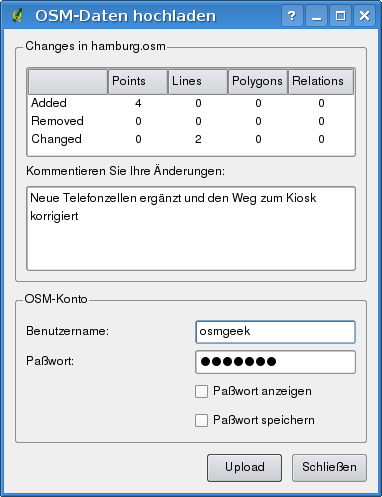
\includegraphics[clip=true, width=8cm]{osm_uploaddialog}
   \caption{OSM upload dialog \nixcaption}\label{fig:osmupload}
\end{figure}

At the top of the dialog you can check, if you are uploading the correct data.
There is a short name of a current database. In the table you find information
on how many changes will be uploaded. Statistics are displayed separately
for each feature type.

In the 'Comment on your changes' box you can write brief information on
meaning of your upload operation. Just write in brief what data changes
you've done or let the box empty.
Fill 'OSM account' arrays so that the server could authenticate you. If
you don't have an account on the OSM server, it's the best time to create
one at \url{http://www.openstreetmap.org}. Finally use \button{Upload} to
start an upload operation.

\subsection{Saving OSM data}

To save data from a current map extent to an XML file click on the
\toolbtntwo{osm_save}{Save OSM to file} button. If there is no such button,
the OSM toolbar in your QuantumGIS installation is probably disabled. You can
enable it again in \mainmenuopt{Settings} \arrow \mainmenuopt{Toolbars} \arrow
\dropmenuopt{OpenStreetMap}. After clicking on the button a new dialog appears.

\begin{figure}[ht]
   \centering
   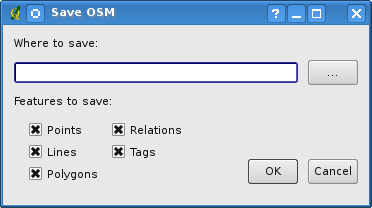
\includegraphics[clip=true, width=8cm]{osm_savedialog}
   \caption{OSM saving dialog \nixcaption}\label{fig:osmsave}
\end{figure}

Select features you want to save into XML file and the file itself. Use
the \button{Ok} button to start the operation. The process will create an
XML file, in which OSM data from your current map extent are represented.
The OSM version of the output file is 0.6. Elements of OSM data
(<node>, <way>, <relation>) do not contain information on their changesets
and uids. This information are not compulsory yet, see DTD for
OSM XML version 0.6. In the output file OSM elements are not ordered.

Notice that not only data from the current extent are saved. Into the output
file the whole polygons and lines are saved even if only a small part of them
is visible in the current extent. For each saved line/polygon all its member
nodes are saved too.

\subsection{Import OSM data}

To import OSM data from an opened non-OSM vector layer follow this
instructions: Choose current OSM data by clicking on one of their layers.
Click on the \toolbtntwo{osm_import}{Import data from a layer} button. If
there is no such button, someone has probably disable the OpenStreetMap
toolbar in your QGIS installation. You can enable it again in
\mainmenuopt{Settings} \arrow \mainmenuopt{Toolbars} \arrow \dropmenuopt{OpenStreetMap}.

After clicking on the button following message may show up:

\begin{figure}[ht]
   \centering
   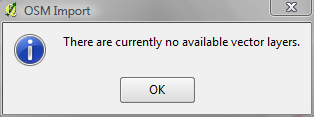
\includegraphics[clip=true, width=8cm]{osm_importdialog}
   \caption{OSM import message dialog \nixcaption}\label{fig:osmimportmessage}
\end{figure}

In such case there is no vector layer currently loaded. The import must be d
one from a loaded layer - please load a vector layer from which you want to
import data. After a layer is opened, your second try should give you a
better result (don't forget to mark the current OSM layer again):

\begin{figure}[ht]
   \centering
   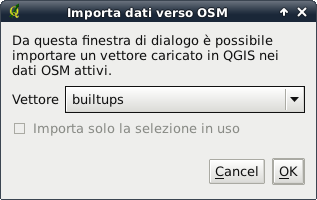
\includegraphics[clip=true, width=8cm]{osm_importtoosmdialog}
   \caption{Import data to OSM dialog \nixcaption}\label{fig:osmimporttoosm}
\end{figure}

Use the submit dialog to start the process of OSM data importing.
Reject it if you are not sure you want to import something.

\FloatBarrier
